\section{Theoretische Grundlagen}

Die Beschreibung von Licht in physikalischen Experimenten hängt von der Betrachtung des Phänomens ab. Grundlegend besteht Licht aus elektromagnetischer Strahlung und erfüllt somit die Maxwell Gleichungen. Für viele 
Experimente genügt bereits eine Betrachtung des Grenzfalls für kleine Wellenlängen. Diese Näherung wird durch die Geometriche Optik beschrieben und kommt vor allem zum Einsatz, wenn keine Wechselwirkung von Strahlung
untereinander betrachtet wird. 
\\
Sichtbar für das menschliche Auge ist Licht mit einer Wellenlänge zwischen $\SI{380}{\nano\meter}$ und $\SI{780}{\nano\meter}$, in diesem Bereich liegen ebenfalls die in dem Versuch verwendeten Laser.
Alle Punkte gleicher Phase bilden eine Wellenfront und die Wellennormale stellt nun den Lichtstrahl in der geometrsichen Optik dar.
Die Ausbreitung der Lichtstrahlen verläuft nach Fermatschen Prinzip geradlinig und ist umkehrbar.
Im folgenden sind zunächst zwei durch die Strahlenoptik beschreibbare Beobachtungen geschildert.

\subsection{Reflexion}
Wenn eine Wellennormale/Lichtstrahl auf eine Grenzfläche fällt, wird diese zum Teil reflektiert. Dabei gilt das Brechungsgesetz \cite{skript}
\begin{equation}
    \label{eqn:tf}
\alpha_{1} = \alpha_{2},
\end{equation}
dabei ist $\alpha_{1}$ der Einfallswinkel auf die Grenzfläche und $\alpha_{2}$ der Reflexionswinkel zum Lot.
\begin{figure}
    \centering
    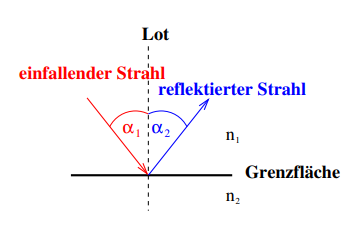
\includegraphics[width=0.4\textwidth]{bilder/1.png}
    \caption{Schematische Abbildung des Reflexionsgesetz von Licht zwischen zwei Medien, getrennt durch eine ebene Grenzfläche. Es gilt dabei die Gleichung \eqref{eqn:tf} und die betrachteten Winkel beziehen sich jeweils auf das Lot, also 
    die Normale der Grenzfläche.\cite{skript}}
    \label{fig:reflexion}
\end{figure}

\subsection{Brechung}
Wichtig für das Verständnis der Brechung ist das Verhalten des Lichts bei Änderung des Trägermediums. Bei einem Übergang zwischen zwei Medien ändert sich sowohl die Geschwindigkeit des Lichts, als auch der Winkel zur Grenzfläche.
Dieses Phänomen lässt sich durch das Snelliussche Brechungsgesetz erklären, dabei gilt \cite{skript}
\begin{equation}
    \label{eqn:snell}
    \frac{\text{sin}\alpha}{\text{sin} \beta} = \frac{v_1}{v_2} = \frac{n_2}{n_1}.
\end{equation}
Der Winkel $\alpha$ gibt den Einfallenden und $\beta$ den ausfallenden Winkel an. Alle Größen mit Index $1$ beschreiben das erste Medium vor der Grenzfläche und der Index $2$ für alle Werte dahinter. Der Brechungsindex $n$ ist die
entscheidende Größe welche angibt wie stark das Licht bei einem Übergang gebrochen wird. Wenn eines der beiden Medien Luft ist vereinfacht sich diese Gesetzmäßigkeit, da der Brechungsindex in Luft $n_{\text{luft}} \approx 1$ ist. Der übrige
Brechungsindex wird dann absolute Brechungsindex genannt.
Wenn $n_2 > n_1$ ist, dann gilt $n_2$ als optisch dichter und die Ausbreitungsgeschwindigkeit ist dort reduziert, anderherum ist $n_2$ optisch dünner, so ist $n_2 < n_1$.
Eine Umformung von Gleichung \eqref{eqn:snell} gibt die bekannte Formulierung des Snelliusschen Brechungsgesetz \cite{skript}
\begin{equation}
n_1 \text{sin}(\alpha) = n_2 \text{sin}(\beta).
\end{equation}
\begin{figure}
    \centering
    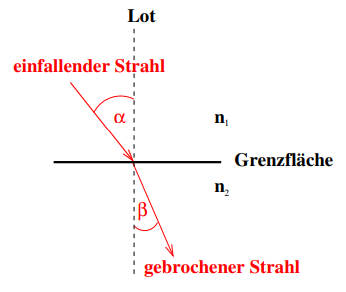
\includegraphics[width=0.4\textwidth]{bilder/2.png}
    \caption{Schematische Abbildung des Brechungsgesetz von Licht zwischen zwei Medien, getrennt durch eine ebene Grenzfläche. Hierbei gilt das Snelliusche Brechungsgesetz \eqref{eqn:snell} und der dargestellte Strahlengang zeigt einen Übergang in ein optisch
    dichteres Medium und die Lichtgeschwindigkeit nimmt hinter Grenzfläche ab.\cite{skript}}
    \label{fig:brechung}
\end{figure}

\subsection{Reflexion und Transmission}
Im allgemeinen wird Strahlung an einer Grenzfläche nicht nur reflektiert sondern auch transmittiert. Da die Intensität allerdings im Optimalfall bei der alleinigen Betrachtung von Transmission und Reflexion nicht verloren geht, gilt das Erhaltungsgesetz
\begin{equation*}
R \cdot T = 1.
\end{equation*}
Die beiden vorherigen Fälle werden miteinader kombiniert.
\begin{figure}
    \centering
    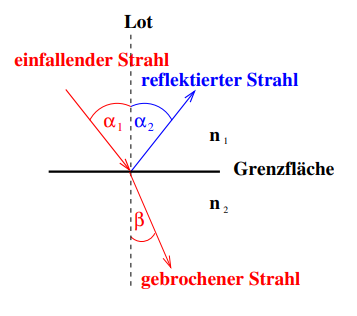
\includegraphics[width=0.4\textwidth]{bilder/3.png}
    \caption{Kombination der Reflexion und Brechung an einer zum Teil durchlässigen Grenzfläche. Es gelten die Gesetzmäßigkeiten wie zuvor. \cite{skript}}
    \label{fig:combo}
\end{figure}

\subsection{Beugung}
Beugung beschreibt das Verhalten von Licht hinter einem Hinderniss, meist einer Blende, wobei die Größenordnung der Öffnung kleiner als die Wellenlänge ist.
Um das Beugungsverhalten von Licht zu verstehen genügt die Strahlenoptik nun nicht mehr. Die Wellenoptik zusammen mit dem Huygenschen Prinzip liefern eine Erklärung. Das Huygensche Prinzip besagt, dass jeder Punkt einer Wellenfront
Ausgangspunkt einer neuen Elementarwelle mit gleicher Frequenz darstellt. Die Einhüllende dieser Elementarwellen stellt nun die neue Wellenfront dar. Dies erklärt warum auch hinter dem Hinderniss Licht erkennbar ist, obwohl es 
nach der Strahlenoptik im Schattenraum liegt. Desweiteren können die Elementarwellen untereinander interferieren da die Maxwellgleichungen die Superposition einzelner Lösungen zulassen. Es kommt zu konstruktiven und destruktiven
Interferenzen hinter einer Blende, abhängig von dem Gangunterschied.